\section{Scope}
\label{sec:scope}

This section describes the scope of the ESMF software. Specific
requirements will be derived from the functionality described here,
and presented in more detail in other requirements documents.

\begin{figure}
  \begin{center}
    \caption{Schematic diagram of ESMF layered architecture.}
    \label{fig:schematic}
    \scalebox{1.0}{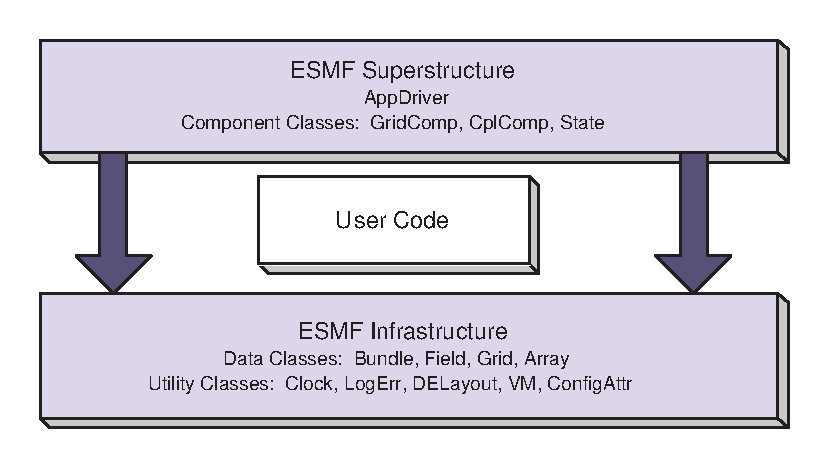
\includegraphics{ESMF_sandwich.eps}}
  \end{center}
\end{figure}

The ESMF provides two primary services: to facilitate coupling of
Earth system model components, and to support lower-level tasks widely
used in Earth Science modeling on high performance computer platforms.
We refer to the first of these services as the ESMF coupling {\it
  superstructure} and the second
as the ESMF utility {\it infrastructure}.\\

\noindent The ESMF consists of:
\begin{itemize}
\item an interface specification for coupling components \footnote{
The science needs of different users
implies a wide variety of continually evolving component interface, for
example Aeolian dust deposition is currently being studied as a
potentially significant process in climate evolution. Ten years ago
almost no atmospheric models or ocean models included these processes,
ten years from now there will almost certainly be other feedbacks to
incorporate. The component interface specification will provide generic
mechanisms, with standard signatures and semantics that support
extensible, flexible and self-describing component model interfaces.
There are conceptual parallels to such Web projects as the
Resource Description Format (http://www.w3.org/RDF). Rather than
attempting to fix domain-wide vocabularies, by enforcing standardized
interfaces, the RDF provides a layer on which
such vocabularies may be expressed, and allowed to evolve. ESMF
component interfaces likewise will provide the bedrock on which specific
component interfaces (e.g an atmospheric model interface) may be expressed.
For example the ESMF interface specification will allow an ocean dynamics component
to indicate that it can provide sea-surface temperature as an output
and will provide a naming mechanism to identify the entities that contain this information. 
Using the ESMF interface specification atmospheric physics and dynamics components 
could then indicate that they require a lower-boundary temperature as an input and 
{\it attach} their lower-boundary temperature inputs to the ocean model sea-surface 
temperature output.
}
; 
\item a complete, portable, high-quality reference implementation
\footnote{
A reference implementation is a widely used approach in deploying open
standards like ESMF. A reference implementation is a product (in this
case a piece of software) that implements a standard. The ESMF reference 
implementation will be fully functional and optimized and will be designed and
tested for use in real applications. The reference implementation for ESMF
will thus be the core framework surce code.
However, it will also serve to
provide other implementors with a standard code to use for validation 
and to use in bootstrapping development of specialized implementations.
Examples of reference implementations of other standards can be found
at http://snad.ncsl.nist.gov/cerberus/,
http://www.socks.nec.com/reference/socks5.html, http://developer.java.sun.com/developer/onlineTraining/J2EE/Intro/,
http://www.netlib.org/blas/, http://www-unix.mcs.anl.gov/mpi/mpich/workingnote/adi2impl/note.html . The Netlib BLAS and MPICH
examples are probably the most familiar to the Earth science community. Most hardware vendors provide platform specialized variants
of these systems. However, these variants are frequently largely derived from the reference codes and are always validated by
comparison against the reference code.
}
  accompanied by extensive developer and user documentation;
\item a suite of application examples demonstrating how the ESMF
  software is used in practice.
\end{itemize}

The model components that the ESMF supports include atmosphere, ocean,
land and sea ice models, and data assimilation systems. Other
well-defined high-level functions may also be represented as
components in the ESMF superstructure.  It is at the level of these
large-scale components that the ESMF interface specification applies
\footnote{
The component interface can be applied to smaller components within a model,
but, the initial development will not deliver then as part of its milestones.
}
.
Each compliant component will provide a specified set of methods that
will enable it to interoperate with other components \footnote{
Extensible, self-describing method interfaces will be used that draw
{\bf conceptually} on the ideas employed by systems for internet
wide interoperability such as RDF - ( see http://www.w3.org/RDF and HTTP)
}
.  For the most
part, we expect components to be able to provide the required
interface functionality through wrapping of internal data structures
and methods. 

\section{ESMF superstructure}
\label{sec:ESMF_superstructure}

All inter-component communication in the framework occurs through 
component calls to the superstructure. Here we provide a synopsis of the
requirements that the superstructure layer will have to meet.
Detailed requirements for the superstructure are given in 
part {\bf \ref{part:Superstructure:_Components}} 
of this document. \\

\noindent The main functions that ESMF superstructure enables (either
directly or through services provided by lower layer functions) are:

\begin{enumerate}
\item any merging, interpolation, or regridding 
of data necessary for communication between components;
\item transferring data between components;
\item sharing attribute information between components;
\item coordinating execution, checkpointing and restarting of
  components.
\end{enumerate}

The superstructure provides a high-level interface that enables 
applications to be assembled from multiple components.  It coordinates
the transfer of distributed grid data and ungridded 
observational data between components.  The superstructure will be able 
to direct the merging of data originating from multiple source grids, and will 
provide spatial and temporal averaging of data (see part {\bf \ref{part:Superstructure:_Components}}
and part {\bf \ref{part:Infrastructure_Fields_and_Grids:_Regridding} }).

The ESMF will be capable of operating in multiple modes of execution.
Components may exist within the same executable, within multiple 
executables, and in mixed modes.  Components may execute serially, 
concurrently, and in mixed modes.

Functionality for regridding, interpolation, redistribution and other 
data communication will be abstracted away from the high-level coupling
interface.  It is provided by a support layer.  
This support layer can be used within components
to perform efficient parallel grid operations.

\section{ESMF infrastructure}
\label{sec:ESMF_infrastructure}

The ESMF contains the software necessary to support the data
decomposition and communication requirements of the superstructure and
individual components.  This includes tools for describing field
data discretized on a wide variety of distributed grids.  The ESMF
supports distributed data operations in a distributed-memory environment, 
in a shared memory environment, and in a hybrid computational environment 
where the platform is a cluster of shared-memory multiprocessors.

\subsection{Fields and grids}

\subsubsection{Fields}
The ESMF supports representation, regridding, and other high-level
collective operations on vector and scalar fields.  A field is represented 
by metadata, a description of its associated distributed grid, and field 
data itself.
The detailed requirements, with formal validation criteria
and relative rankings, for this aspect of ESMF are given
in parts {\bf \ref{part:Infrastructure_Fields_and_Grids:_Physical_Grids} },
{\bf \ref{part:Infrastructure_Fields_and_Grids:_Regridding} }
and 
{\bf \ref{part:Infrastructure_Fields_and_Grids:_Distributed_Grids} } of this document.
Here we provide a brief synopsis of the areas that are covered
in that part of the document.

\subsubsection{Gridded and observational data}

The ESMF supports regridding, interpolation, redistribution,
transfer, and merging of data discretized on the following types of grids:

\begin{enumerate}
\item logically rectilinear grids: physical co-ordinates may be
  curvilinear. Logically rectilinear grids include such grids as the
  tripolar and the cubed sphere;
\item reduced and regional grids;
\item unstructured grids (e.g., land grids);
\item phase space grids (e.g., spectral, Fourier);
\item nested grids;
\item observational data streams (temporal sequences of ungridded data);
\item other grids (e.g icosahedral).
\end{enumerate}


The supplied implementation will include highly-optimized versions of
these operations for the commonly-used and representative grid types. The detailed 
requirements for this aspect of ESMF of given in parts 
{\bf \ref{part:Infrastructure_Fields_and_Grids:_Physical_Grids} } ({\it Physical Grids}
detailed requirements - which deals with what continuous spaces and disrete forms
need to be represented) and 
{\bf \ref{part:Infrastructure_Fields_and_Grids:_Distributed_Grids} } 
({\it Distributed Grids} detailed requirements - which deals with parallel representations
of these grids)
of this document.
The detailed requirements include explicit requirements for future extensibility mechanisms to allow
support for other grids to be easily introduced.

\subsubsection{Grid operations}

The ESMF provides interpolation algorithms for supported grids.  
The detailed requirements, with formal validation criteria
and relative rankings, for this aspect of ESMF are given
in part {\bf \ref{part:Infrastructure_Fields_and_Grids:_Regridding}}.
Here we provide a brief synopsis of the areas that are covered
in that part of the document.
All interpolation algorithms included in ESMF are {\it linear} in the data
and will be accompanied by the associated adjoint.  Adaptive
procedures are not planned at this stage. Thus, reconstruction of
gridded data from observations (analysis) will not be a part of
framework and will rather be provided by data assimilation components.

The ESMF provides first-order and higher-order interpolation 
methods.  The ESMF supports conservative remapping/interpolation 
between any two grids. Non-conservative methods will also 
be supported.

Dynamic load balancing will be provided for standard decompositions, 
and general dynamic load-balancing tools for specialized decompositions.

\subsection{Utility infrastructure}
The ESMF includes general purpose utility routines for use by both 
the ESMF coupler and application codes.
The detailed requirements, with formal validation criteria
and relative rankings, for this aspect of ESMF are given
in parts {\bf \ref{part:Infrastructure_Utilities:_Time_Management}} -
 {\bf \ref{part:Infrastructure Utilities:_I/O}} of this document.
Here we provide a brief synopsis of the areas that are covered
in that part of the document.
These utilities, described in parts {\bf \ref{part:Infrastructure_Utilities:_Time_Management}} to 
{\bf \ref{part:Infrastructure Utilities:_I/O}},
include but are not limited to:
\begin{enumerate}
\item communication primitives (see part {\bf \ref{part:Infrastructure_Utilities:_Communication_and_Memory_Kernels}});
\item a generic machine interface (see part {\bf \ref{part:Infrastructure_Utilities:_Communication_and_Memory_Kernels}});
\item I/O utilities (see part {\bf \ref{part:Infrastructure Utilities:_I/O}};
\item general message logging (see part {\bf \ref{part:Infrastructure_Utilities:_Log}});
\footnote{Like many other elements under
{\it Utility infrastructure}, the querying and publishing functions will be 
fundamental to the superstructure control and coupling areas. Isolating the
requirements here does not imply a particular system design organization
or ranking.
}
\item performance profiling (see part {\bf \ref{part:Infrastructure_Utilities:_Performance_Profiling}});
\item time management (see part {\bf \ref{part:Infrastructure_Utilities:_Time_Management}}); and
\item error handling (see \ref{req:gr:error_handling} and part {\bf \ref{part:Infrastructure_Utilities:_Log}}).
\end{enumerate}

\subsubsection{Communication primitives}

ESMF will offer a standard interface covering inter-processor
communication and shared address space primitives, covering
point-to-point communication, global reduction operations, etc. An
implementation in MPI will be provided.

\subsubsection{Generic machine interface}

ESMF will offer a generic interface to hardware, O/S and system
library primitives.

\subsubsection{I/O}

The ESMF I/O utilities will include generic interfaces providing I/O
in a variety of data formats including netCDF, HDF, binary, GRIB, and
BUFR. As much as possible, the utilities will offer scalable, parallel I/O,
performance.

\subsubsection{Performance profiling}

A performance profiling utility will enable application developers to 
instrument code segments with timers. The profiling utility will also
offer access to hardware statistics by offering an interface to a
package such as PAPI or PCL.

\subsubsection{Time management}

The ESMF will include a library for performing routine 
calculations with dates and time intervals.  For higher level model
time management, the ESMF will include clocks for advancing and 
reporting model time and retaining model integration information, 
and alarms for initiating both unique and periodic events.

\subsubsection{Error handling}

The ESMF will offer comprehensive and integrated error handling
services.  A mechanism to announce and query component failure will be
provided.

\subsection{Future plans}

The following are capabilities that might conceivably have been
included in ESMF, but will not be developed under CAN 00-OES-01
funding:
\begin{enumerate}
\item a Graphical User Interface;
\item mathematical libraries for operations other than regridding and
  interpolation;
\item standard scientific modules, such as a library for calculating
  orbital parameters;
\item a database of intra-model components, such as convection schemes;
\item a database for storing experiments and related information;
\item a mechanism for job submission (e.g Globus);
\item optimization for additional model grids.
\end{enumerate}

If additional resources are made available, the ESMF project foresees
extending the initial framework.  Each of the features listed above is
a possible addition.




















